\chapter{}
Sou do tempo bom em que os adultos se livravam das crianças sem culpa, mandando: “Vão brincar lá fora!”.
E “lá fora” era o quintal, o maravilhoso país da infância.
Sobretudo quando se vivia numa cidade do interior. 
Era o espaço de descobrir e pensar o mundo. 
Observar as formigas na sua labuta incessante, as lagartixas subindo pelo velho muro meio rachado, as borboletas iridescentes, o rastro prateado e gosmento desenhado pelos vagarosos caracóis.   
Contemplar a incessante migração das nuvens que o vento ora esfiapava, ora ia juntando em formas caprichosas de bichos, árvores, gigantes, castelos, anjos e às vezes mapas, como aqueles pendurados nas paredes da sala de aula. 
Sentir o cheiro da roupa lavada e embebida de sol, pendurada no varal; da fumaça desprendendo-se da lenha queimada no fogão; da terra molhada, da moita de arruda, das rosas, do jasmim, do manacá; do bafio úmido de sepulcro que emanava da escura caverna do porão. 
Deitada de costas nas pedras quentes da calçada, abandonava-me ao sol. O calor invadia aos poucos meu corpo, amolecendo braços e pernas e eu os imaginava penetrando terra adentro, como raízes. 
Imóvel, escutava o zunido das abelhas nas flores, os recados insistentes do “fogo apagou” e do bem-te-vi vindos lá das bandas do cemitério, o canto dos sabiás e a algazarra dos pardais e andorinhas sobrevoando a velha paineira do almoxarifado da prefeitura bem ali, do outro lado da rua. 
Na marcenaria, alguns quarteirões acima, o som plangente da serra cortando madeira dividia com o sino da torre da Matriz a tarefa de marcar regularmente a passagem das horas. 
Vez ou outra, roncando em agonia a cada mudança de marcha, os velhos ônibus a querosene passavam sacolejando nos paralelepípedos, rua acima; os carros ainda eram raros. 
E, do outro lado do muro, do barracão da fábrica do meu pai, chegava o som oceânico, abafado e constante das máquinas torcendo os fios de algodão para transformá-los nos novelos de barbante que garantiam o sustento da nossa família e a minha doce vadiagem de criança.

As cores, formas e textura das flores e folhagens me fascinavam. 
Recobriam meus desenhos infantis e emolduravam em cercaduras delirantes as páginas dos meus cadernos de escola.

Na opinião da minha mãe, as flores do nosso quintal deviam obedecer à moda, como tudo o mais. 
Lembro-me da fase dos crisântemos, dálias e crisandálias repolhudas, logo repudiadas em favor das rosas que, por sua vez, acabaram arrancadas para dar lugar às palmas de Santa Rita e às gérberas. 
Essas mudanças eram quase sempre decididas por volta do Dia de Finados, quando as parentes da Capital chegavam sobraçando as novidades compradas nas floriculturas do Arouche. 
Houve uma vez em que a matriarca das hostes paulistanas, Tia Angelina, desceu do trem exibindo buquês de soberbos e inacreditáveis gladíolos azuis. Foi o quanto bastou para que as nossas pobres palmas de Santa Rita caíssem em desgraça. 
“Coisa mais calú!”, decretou minha mãe. 
Era sua expressão favorita para o que lhe parecia vulgar ou caipira. O projeto do novo jardim teve, porém, que ser adiado. 
De tanto mexer na terra, nas sucessivas reformas dos nossos canteiros, mamãe arrumou uma infecção persistente nos dedos que acabou por lhe fazer caírem as unhas. 
Até um médico especialista em São Paulo precisou ser consultado, já que o nosso habitual curandeiro, o Joãozinho da Farmácia, amigo de longa data do papai, não conseguiu resolver a tal eczema.

De qualquer modo, outros e mais amplos planos de mudança começavam a agitar minha família, pois mamãe começara a achar “calús” não só as flores, como todo o quintal, a casa antiga de “parede a meia” e banheiro fora, os móveis escuros, “art-déco”. 
Papai prosperava nos negócios e mamãe já podia sonhar mais alto: uma casa moderna, com mais cômodos, armários embutidos, num bairro novo e mais nobre. 
Prenunciando a nova fase, nossa antiga sala de jantar desapareceu para dar lugar a uma mobília nova e aromática, de jacarandá torneado, em que se destacava uma vistosa cristaleira apropriadamente recheada com copos de cristal recém-adquiridos e que tilintavam perigosamente a cada passo nosso sobre o velho assoalho. 
Nossas caminhas \textit{Patente} foram substituídas por outras, artisticamente torneadas também e os velhos colchões de crina foram para o lixo. 
Passamos a dormir em modernos colchões de mola. Um tapeceiro alemão veio tirar as medidas para fabricar sofá, poltrona e cortinas para a sala de estar. 
Coroando todo esse luxo, um dia desembarcou em nosso portão a peça central da nova decoração: um piano de nogueira, novo em folha, que se converteria num dos grandes instrumentos de tortura da minha juventude. 
Porque então, junto com o quintal e a velha casa, ficava para trás também a minha infância. 
Eu me tornara uma adolescente e, em breve, nós mudaríamos para a casa da Av. D. Pedro II, n.º 1273, defronte ao Clube de Campo do Araraquarense. Corria o ano de 1958.

\begin{figure}[H]
\centering
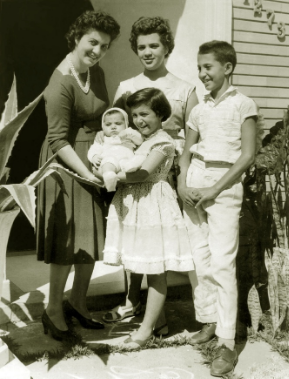
\includegraphics[width=0.5\linewidth]{1/maria-joão.png}
\caption{A família na porta da casa nova. No colo da
Maria Lúcia, o recém-chegado João.}
\end{figure}